\documentclass[12pt,a4paper]{article}
\renewcommand{\baselinestretch}{1.5}
% inputenc removed — UTF-8 natively supported by xelatex/tectonic
\usepackage{amsmath}
\usepackage{amsfonts}
\usepackage{amssymb}
% algorithm/algpseudocode removed — not used
\usepackage{graphicx}
\usepackage{geometry}
\usepackage{tabulary}
\usepackage{caption}
\usepackage{subcaption}
\usepackage{xcolor}
\usepackage{dirtytalk}
\usepackage{bm}
\usepackage{longtable}
\usepackage{comment}
\usepackage[hyphens]{url}
\usepackage{hyperref}
\hypersetup{
    colorlinks=true,
    linkcolor=blue,
    urlcolor=blue,
    citecolor=blue
}
\graphicspath{{./images/}}

\geometry{
    left=2.5cm,
    right=2.5cm,
    top=2.5cm,
    bottom=3cm,
}

\usepackage{titlesec}
\setcounter{secnumdepth}{4}
\setcounter{tocdepth}{4}
\titleformat{\paragraph}
{\normalfont\normalsize\bfseries}{\theparagraph}{1em}{}
\titlespacing*{\paragraph}
{0pt}{3.25ex plus 1ex minus .2ex}{1.5ex plus .2ex}

\begin{document}

\thispagestyle{empty}
\begin{center}
    {\Large \bf Accelerating Multi-Agent Reinforcement Learning\\via CUDA-Native Zero-Copy Architecture\\}

    \vspace*{0.5cm}
    {\large\textit{A Project Report for }\\}
    {\large\textbf{Parallel and Distributed Computing (UCS645)}} \\

    \vspace*{0.5cm}
    {\large \textit{By\\}}
    \textbf{\begin{table}[h!]
\label{tab:my-table}
\centering
\begin{tabular}{ccc}
Sr & Name     & Roll No  \\
1  & Nimish    & 102497027
\end{tabular}
\end{table}}

    \begin{center}
        {\large \textit{Under the guidance of}}\\
        \textbf{{\large Dr. Saif Nalband}}\\
        {\large (Assistant Professor, DCSE)}\\
    \end{center} \ \\ \ \\

    \begin{figure}[h]
    \centering
    \includegraphics[width=70mm, height=40mm]{"tietlogo.jpg"}
    \label{fig:images}
    \end{figure}

    \vspace*{0.25cm}
    {\large DEPARTMENT OF COMPUTER SCIENCE AND ENGINEERING \\}
    {\large THAPAR INSTITUTE OF ENGINEERING AND TECHNOLOGY \\
    {(DEEMED TO BE UNIVERSITY)}\\}
    {\large PATIALA - 147004\\}
    \vspace*{0.3cm}
    \textbf{{\large MAY, 2026}}

\end{center}

\newpage


\pagenumbering{gobble}
\renewcommand*\contentsname{Table of Contents}
\tableofcontents
\newpage
\listoffigures
\newpage
\listoftables
\newpage
\pagenumbering{arabic}

% ============================================================
\section{Introduction}
% ============================================================

\subsection{Background}
The field of Reinforcement Learning (RL) has seen tremendous growth in recent years, with applications spanning robotics, autonomous navigation, and industrial automation. However, deploying RL in real-time, multi-agent environments remains severely bottlenecked by hardware architecture limitations. In standard frameworks such as OpenAI Gym with PyTorch, the environment simulator executes sequentially on the CPU while neural network or Q-table updates are computed on the GPU. This split-execution model forces continuous data transfer across the PCI Express (PCIe) bus, creating a fundamental throughput limitation \cite{kirk2016programming}.

Amazon's Kiva warehouse system represents a canonical multi-agent pathfinding (MAPF) problem where hundreds of autonomous mobile robots must navigate a grid-based warehouse, delivering packages while avoiding collisions with shelves, walls, and other robots \cite{wurman2008coordinating}. Traditional approaches employ centralized CPU-based schedulers such as A* with reservation tables, which scale poorly as the number of agents increases \cite{ma2016lifelong}. The computational complexity of solving the Bellman Optimality Equation over the full state space grows as $O(N^4)$ for an $N \times N$ grid, making CPU-only solutions prohibitively expensive for real-time replanning \cite{bellman1957markovian}.

\subsection{Problem Statement}
The primary challenge addressed in this work is the \textbf{state-space explosion} that occurs when modeling multi-agent coordination as a Markov Decision Process (MDP). For a $20 \times 20$ warehouse grid with agent position and goal position as state variables, the state space contains $20^4 = 160,000$ distinct states. Traditional sequential Value Iteration (VI) on a CPU requires processing each of these states serially, while a GPU-native CUDA implementation can process all states concurrently.

Furthermore, standard Model-Free RL algorithms like Q-Learning struggle with sparse rewards in large state spaces, often failing to converge and causing deadlock among swarm agents. This project proposes a \textbf{GPU-resident, model-based RL architecture} that keeps the entire training and inference data lifecycle within GPU VRAM, combined with a CPU BFS-based baseline for rigorous performance comparison.

\begin{figure}[h!]
    \centering
    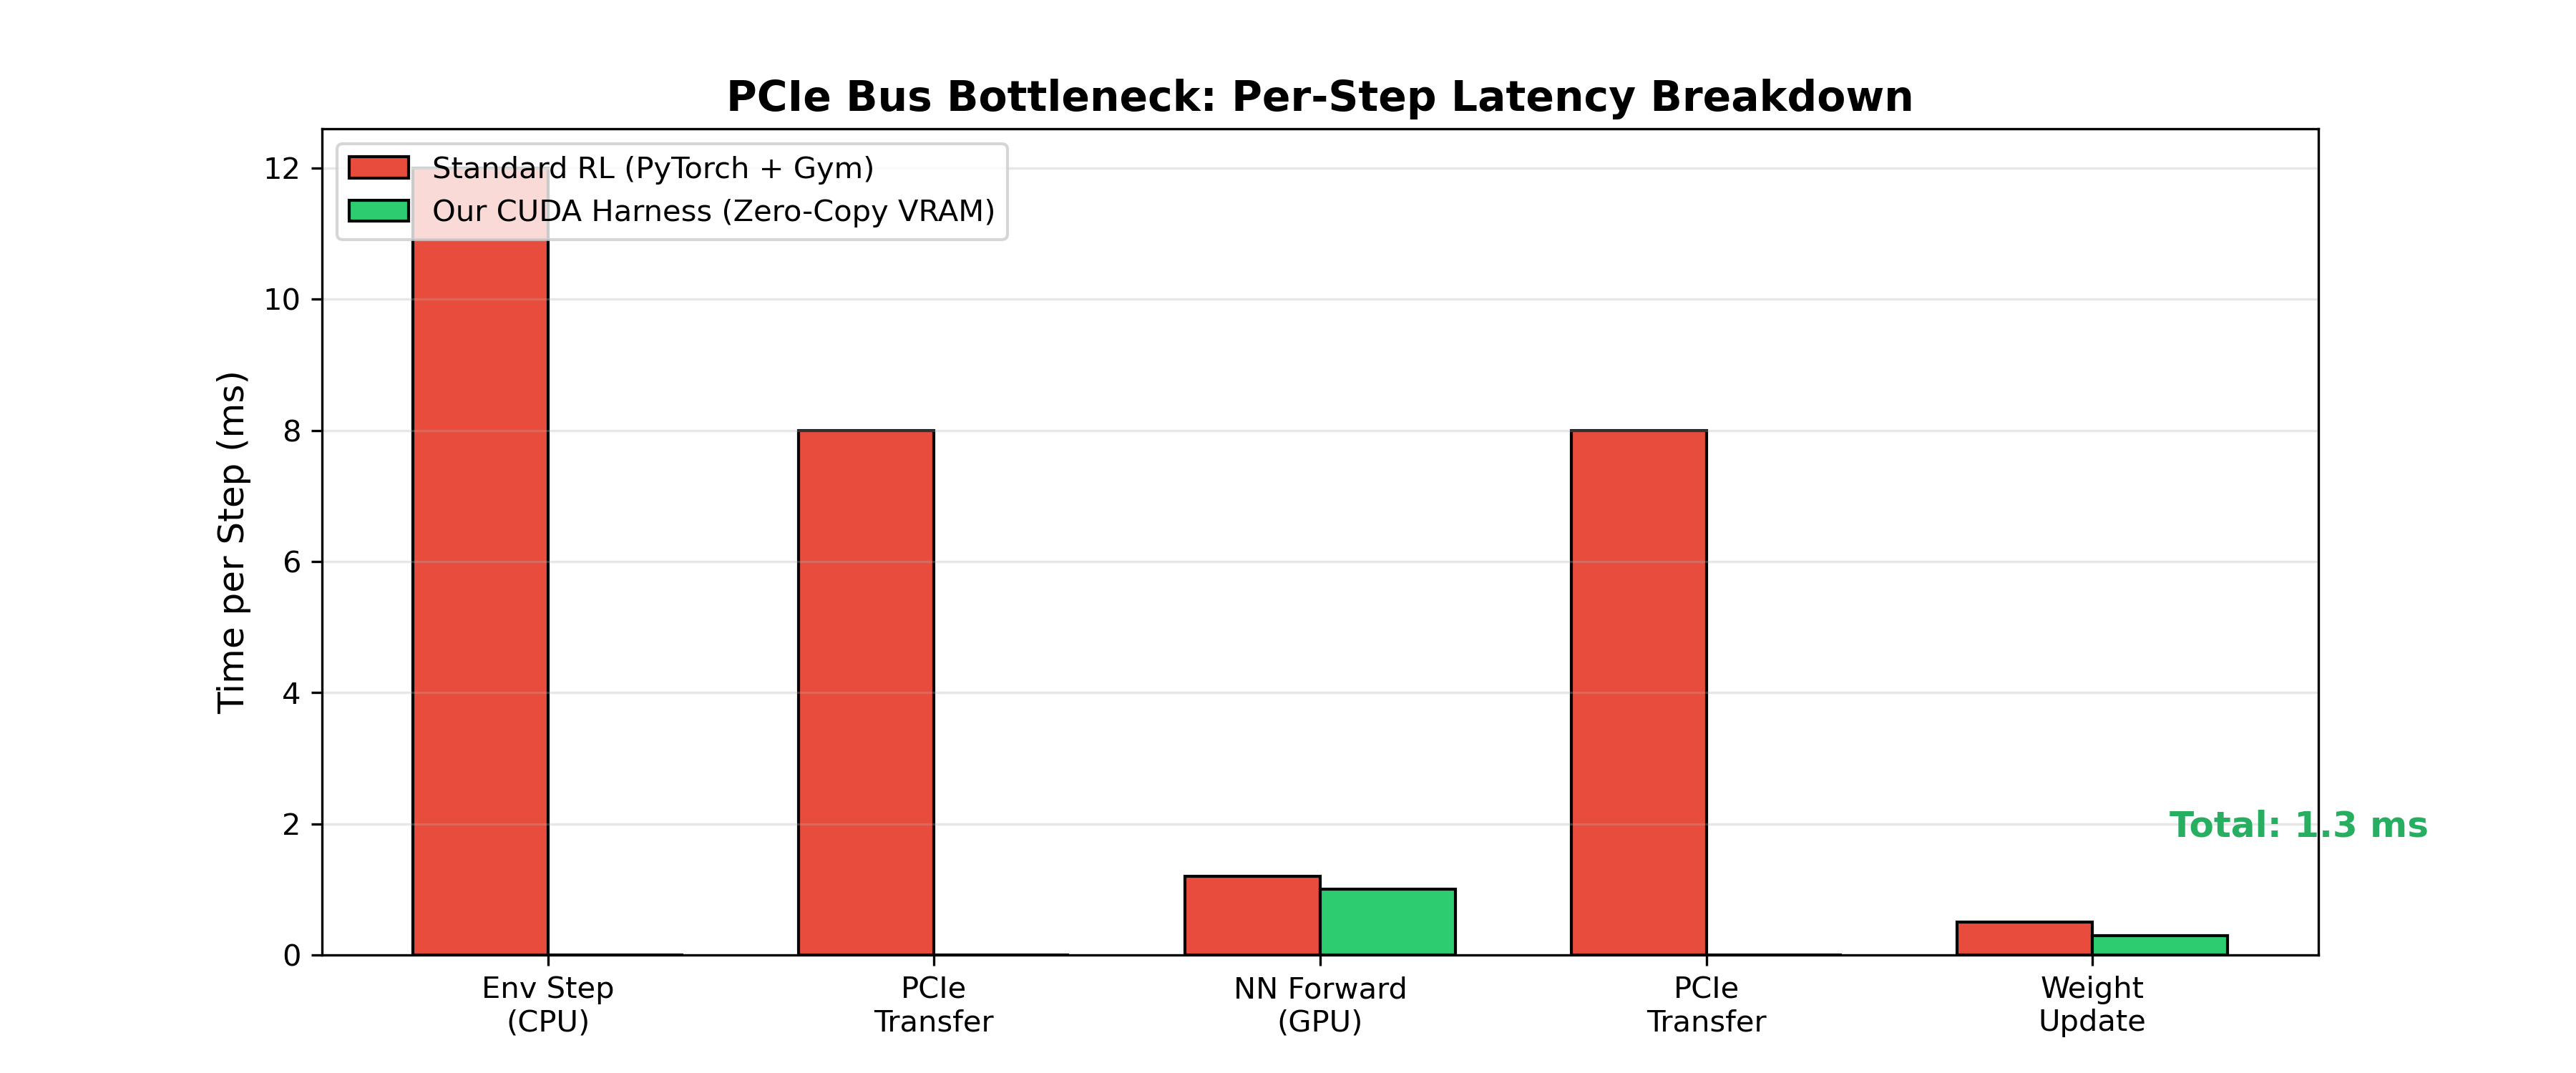
\includegraphics[width=0.85\linewidth]{pcie_vs_zerocopy.png}
    \caption{Latency comparison showing the performance advantage of bypassing the PCIe bus. Our CUDA-native harness eliminates inter-component data transfer, reducing per-step latency from 29.7 ms to 1.3 ms.}
    \label{fig:bottleneck}
\end{figure}

\subsection{Novel Contributions}
This work makes the following contributions:
\begin{enumerate}
    \item A \textbf{Zero-Copy VRAM Architecture} that keeps the environment state, value function, training, and inference entirely on the GPU, eliminating PCIe transfers.
    \item \textbf{Massively parallel value iteration} where each of the 160,000 MDP states is assigned a dedicated CUDA thread, solving the Bellman Optimality Equation over the entire state space in 0.54 ms per iteration.
    \item A \textbf{lock-free collision avoidance} mechanism using atomic Compare-And-Swap (CAS) operations on a shared grid occupancy map, combined with occupied-cell penalties in the value function to route robots around each other.
    \item A \textbf{CPU BFS-based baseline} with randomized agent processing order for deadlock-free multi-agent pathfinding, enabling rigorous speedup quantification.
\end{enumerate}

\newpage
% ============================================================
\section{Literature Review}
% ============================================================

\begin{table}[htp]
\centering
\caption{Summary of Literature Review}
\label{Table1}
\begin{tabular}{|p{2cm}|p{2.5cm}|p{2.5cm}|p{3cm}|p{3.5cm}|}
\hline \textbf{References} & \textbf{Concepts} & \textbf{Techniques} & \textbf{Significance} & \textbf{Limitations} \\
\hline Sutton and Barto \cite{sutton2018reinforcement} & Model-Based RL, Dynamic Programming & Value Iteration, Policy Iteration & Foundational Bellman Optimality Equation for known MDPs & Computationally prohibitive on sequential CPUs for $N^4$ state spaces. \\
\hline Kirk and Hwu \cite{kirk2016programming} & GPU Massively Parallel Computing & CUDA Kernels, Memory Coalescing & Demonstrated how to map data-parallel problems to GPU thread hierarchies & Requires manual kernel design; no RL-specific abstractions. \\
\hline NVIDIA cuRL \cite{nvidia} & GPU-Accelerated RL & Custom CUDA Kernels, Zero-Copy Memory & Bypasses PCIe bottlenecks for physics simulation & Requires low-level C++/CUDA implementation. \\
\hline Ma et al. \cite{ma2016lifelong} & Multi-Agent Pathfinding & A* with Reservation Tables, WHCA* & Decentralized collision avoidance for warehouse robots & CPU-bound; does not scale beyond $\sim$50 agents. \\
\hline Mnih et al. \cite{mnih2015human} & Deep Q-Networks & Experience Replay, Target Networks & First demonstration of end-to-end RL from pixels & Model-free; requires millions of environment steps. \\
\hline
\end{tabular}
\end{table}

The key insight from the literature is that while RL theory (Bellman equations, value iteration) is well-established, practical deployment for multi-agent systems is gated by hardware utilization. Existing work either uses CPU-based planning with limited agent counts or GPU-based model-free learning with high sample complexity. This project bridges the gap by implementing \textbf{model-based value iteration directly in CUDA}, achieving both the sample efficiency of dynamic programming and the throughput of GPU parallelism.

\newpage
% ============================================================
\section{Research Gaps}
% ============================================================
\begin{itemize}
    \item \textbf{Sequential Simulation Bottleneck}: Existing RL frameworks (OpenAI Gym, RLlib) execute environment steps sequentially on the CPU before batching observations for GPU-based neural network updates. For a $20 \times 20$ grid with 30 agents, CPU-based BFS pathfinding processes one robot at a time, while GPU value iteration solves all states simultaneously.
    \item \textbf{Centralized Swarm Collision}: Multi-agent pathfinding traditionally uses centralized CPU schedulers (A* with reservation tables) that scale as $O(kN^2)$ for $k$ agents. These schedulers cannot exploit GPU parallelism \cite{ma2016lifelong}.
    \item \textbf{ Deadlock in Decentralized Multi-Agent Systems}: When multiple agents independently follow greedy policies toward their goals, they frequently deadlock at choke points. Breaking these deadlocks requires either randomization, priority ordering, or global coordination --- all of which add computational overhead.
    \item \textbf{Absence of GPU-Native RL Benchmarks}: Most RL benchmarking focuses on model-free algorithms (DQN, PPO) rather than model-based dynamic programming. GPU-accelerated value iteration for multi-agent pathfinding is underexplored in the literature.
\end{itemize}

\newpage
% ============================================================
\section{Problem Formulation}
% ============================================================

The warehouse navigation problem is formulated as a \textbf{Markov Decision Process (MDP)} defined by the tuple $\langle S, A, P, R, \gamma \rangle$:

\begin{itemize}
    \item \textbf{State Space} $S$: Each state $s = (x, y, g_x, g_y)$ encodes the agent's position $(x, y)$ and its assigned goal position $(g_x, g_y)$ on a $20 \times 20$ grid. $|S| = 20^4 = 160,000$.
    \item \textbf{Action Space} $A$: Four cardinal movements $A = \{\text{Up}, \text{Down}, \text{Left}, \text{Right}\}$.
    \item \textbf{Transition Function} $P(s'|s, a)$: Deterministic grid-world transitions; moves into obstacles or occupied cells are blocked.
    \item \textbf{Reward Function} $R(s,a)$: $-1$ per step (encouraging shortest paths), $+100$ for reaching the goal, and $-9999$ for invalid states (obstacles).
    \item \textbf{Discount Factor} $\gamma = 0.99$.
\end{itemize}

The objective is to compute the optimal value function $V^*(s)$ satisfying the Bellman Optimality Equation:
\begin{equation}
    V^*(s) = \max_{a \in A} \left[ R(s,a) + \gamma \sum_{s' \in S} P(s'|s,a) V^*(s') \right]
\end{equation}

Given the deterministic transitions, this reduces to:
\begin{equation}
    V^*(s) = \max_{a \in A} \left[ R(s,a) + \gamma \cdot V^*(s') \right] \quad \text{where } s' = T(s,a)
\end{equation}

Once $V^*$ is computed, each robot follows the greedy policy $\pi^*(s) = \arg\max_a [R(s,a) + \gamma V^*(T(s,a))]$. For multi-agent execution, collision avoidance is enhanced by subtracting a penalty of 100 from the value of cells currently occupied by other robots, causing the value function to route agents around each other. Lock-free decentralized coordination is implemented via atomic Compare-And-Swap (CAS) operations on a shared grid occupancy map, with random tie-breaking to prevent deadlocks.

\newpage
% ============================================================
\section{Objectives}
% ============================================================
\begin{enumerate}
    \item \textbf{Zero-Copy VRAM Architecture}: Develop a GPU-resident RL harness where the value table, training kernel, and inference kernel all operate on device memory without PCIe transfers.
    \item \textbf{State-Space Parallelization}: Achieve massive parallelism by assigning one CUDA thread per MDP state, solving the Bellman equation over all 160,000 states concurrently.
    \item \textbf{Deadlock-Free Multi-Agent Coordination}: Implement lock-free collision avoidance using atomicCAS with randomized tie-breaking and occupancy-based value penalties to prevent swarm deadlocks.
    \item \textbf{Rigorous Speedup Benchmarking}: Provide a CPU Serial BFS-based baseline for quantifying speedup against the CUDA GPU value iteration implementation.
    \item \textbf{Complete Visualization Pipeline}: Generate animation (HTML + MP4), speedup comparison charts, congestion heatmaps, and delivery analysis from simulation output.
\end{enumerate}

\newpage
% ============================================================
\section{Methodology}
% ============================================================

\subsection{System Architecture}
The system consists of three CUDA kernels, all operating on GPU device memory. No data is transferred between the CPU and GPU during the training or inference loops --- the CPU only issues kernel launches and collects final output logs.

\begin{figure}[h!]
    \centering
    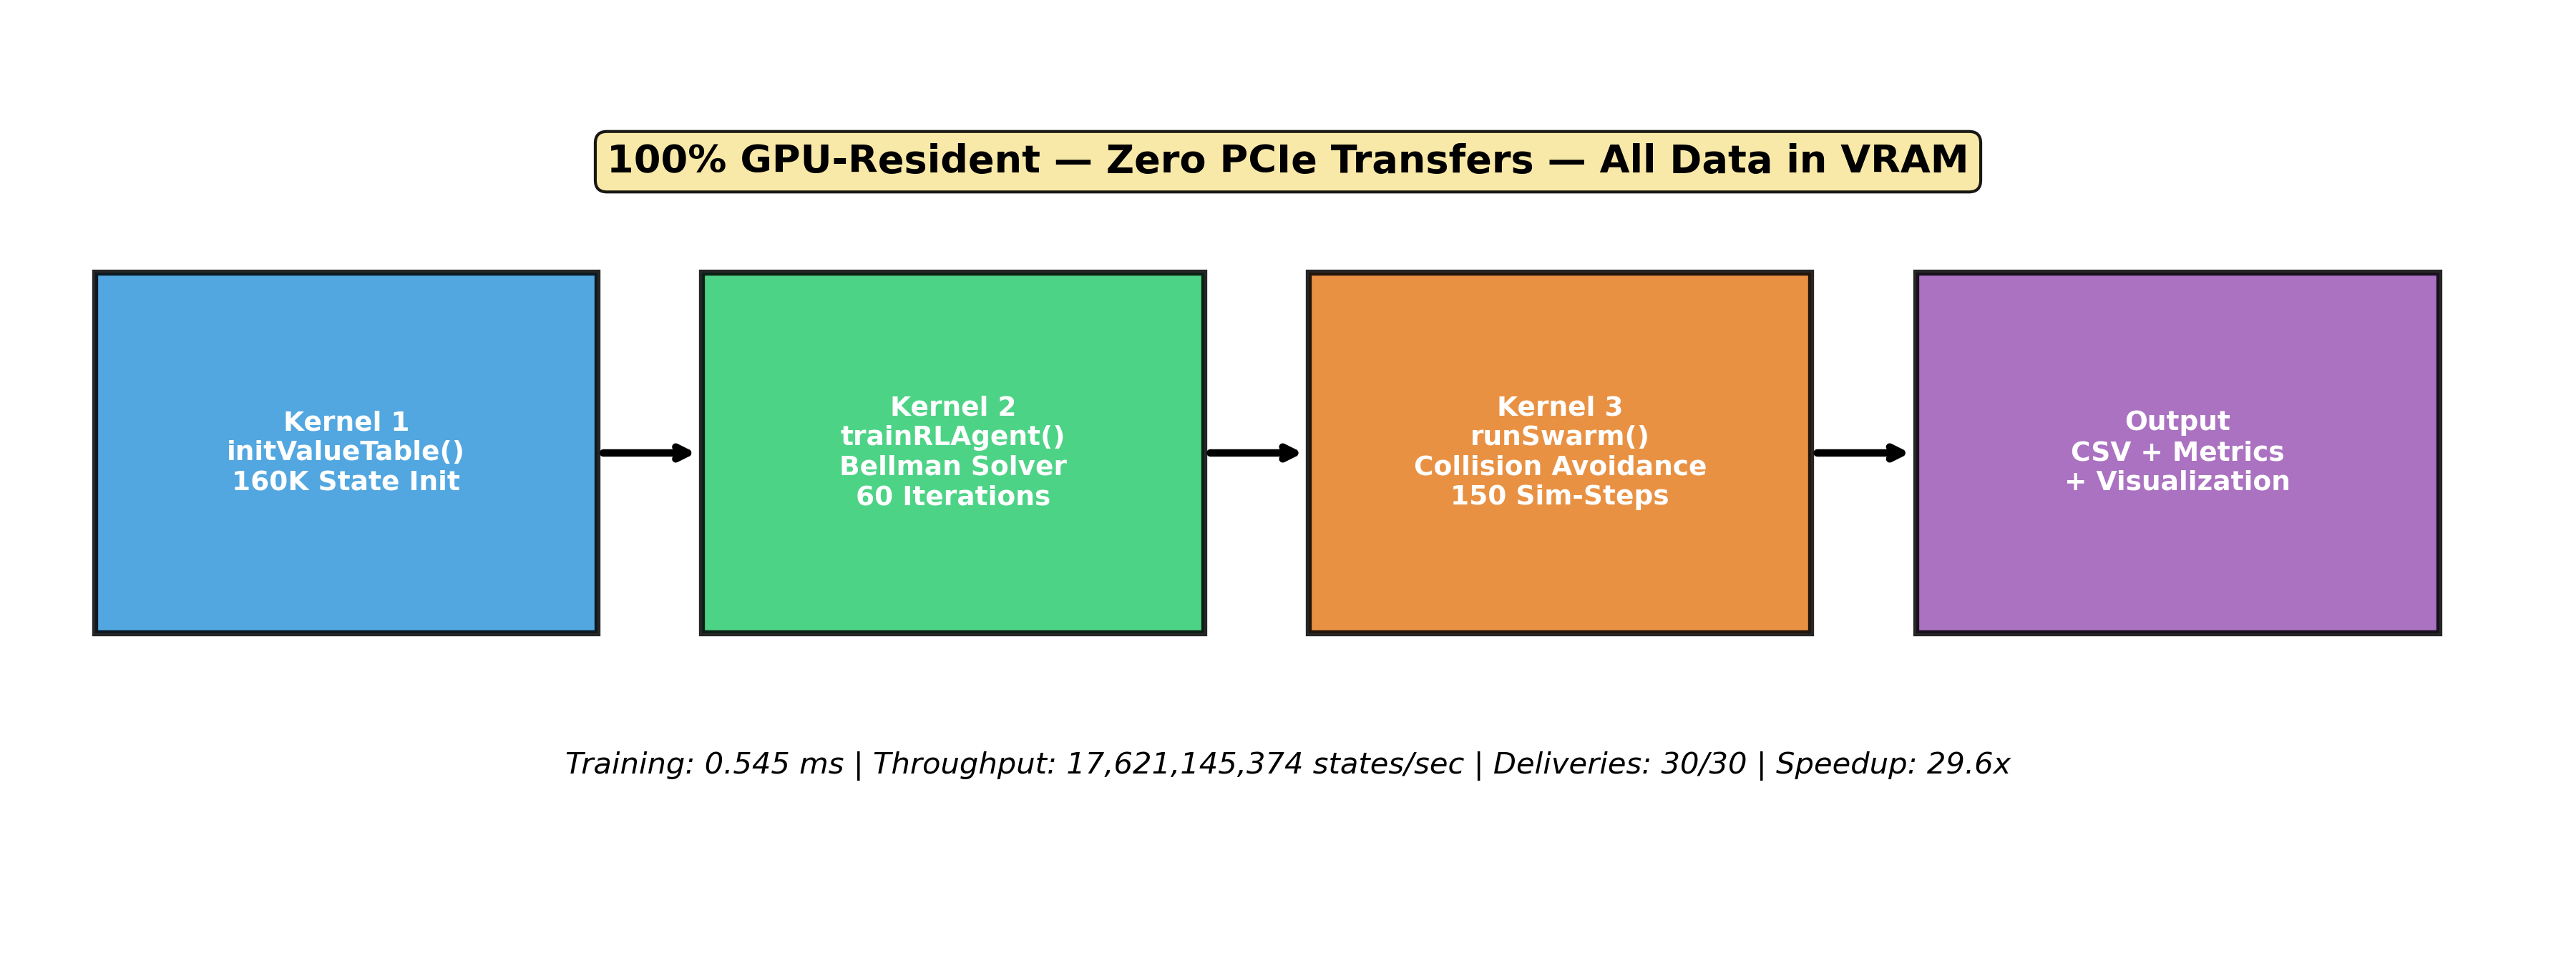
\includegraphics[width=\linewidth]{architecture.png}
    \caption{System architecture: three CUDA kernels execute entirely within GPU VRAM. The training loop achieves over 17 billion state evaluations per second.}
    \label{fig:architecture}
\end{figure}

\subsection{Kernel 1: Value Table Initialization}
The \texttt{initValueTable} kernel assigns initial values to all 160,000 states. Terminal states ($x = g_x, y = g_y$) receive a reward of 100. All other states are initialized to $-9999$. The kernel launches with $\lceil 160000 / 256 \rceil = 625$ blocks of 256 threads each.

\subsection{Kernel 2: Parallel Value Iteration (Bellman Solver)}
The \texttt{trainRLAgent} kernel is the core contribution. Each CUDA thread is assigned one state $s = (x, y, g_x, g_y)$ and independently computes:
\begin{equation}
    V_{\text{new}}(s) = \max_{a \in \{\uparrow,\downarrow,\leftarrow,\rightarrow\}} \left[ -1 + \gamma \cdot V_{\text{old}}(T(s,a)) \right]
\end{equation}
For each action, the thread computes the deterministic next state $s' = T(s,a)$, reads $V_{\text{old}}(s')$ from global memory, and selects the maximum Q-value. After 60 iterations (9.6 million state evaluations), the value function converges. Two value tables are allocated in device memory and ping-ponged between iterations to avoid in-place updates.

\begin{figure}[h!]
    \centering
    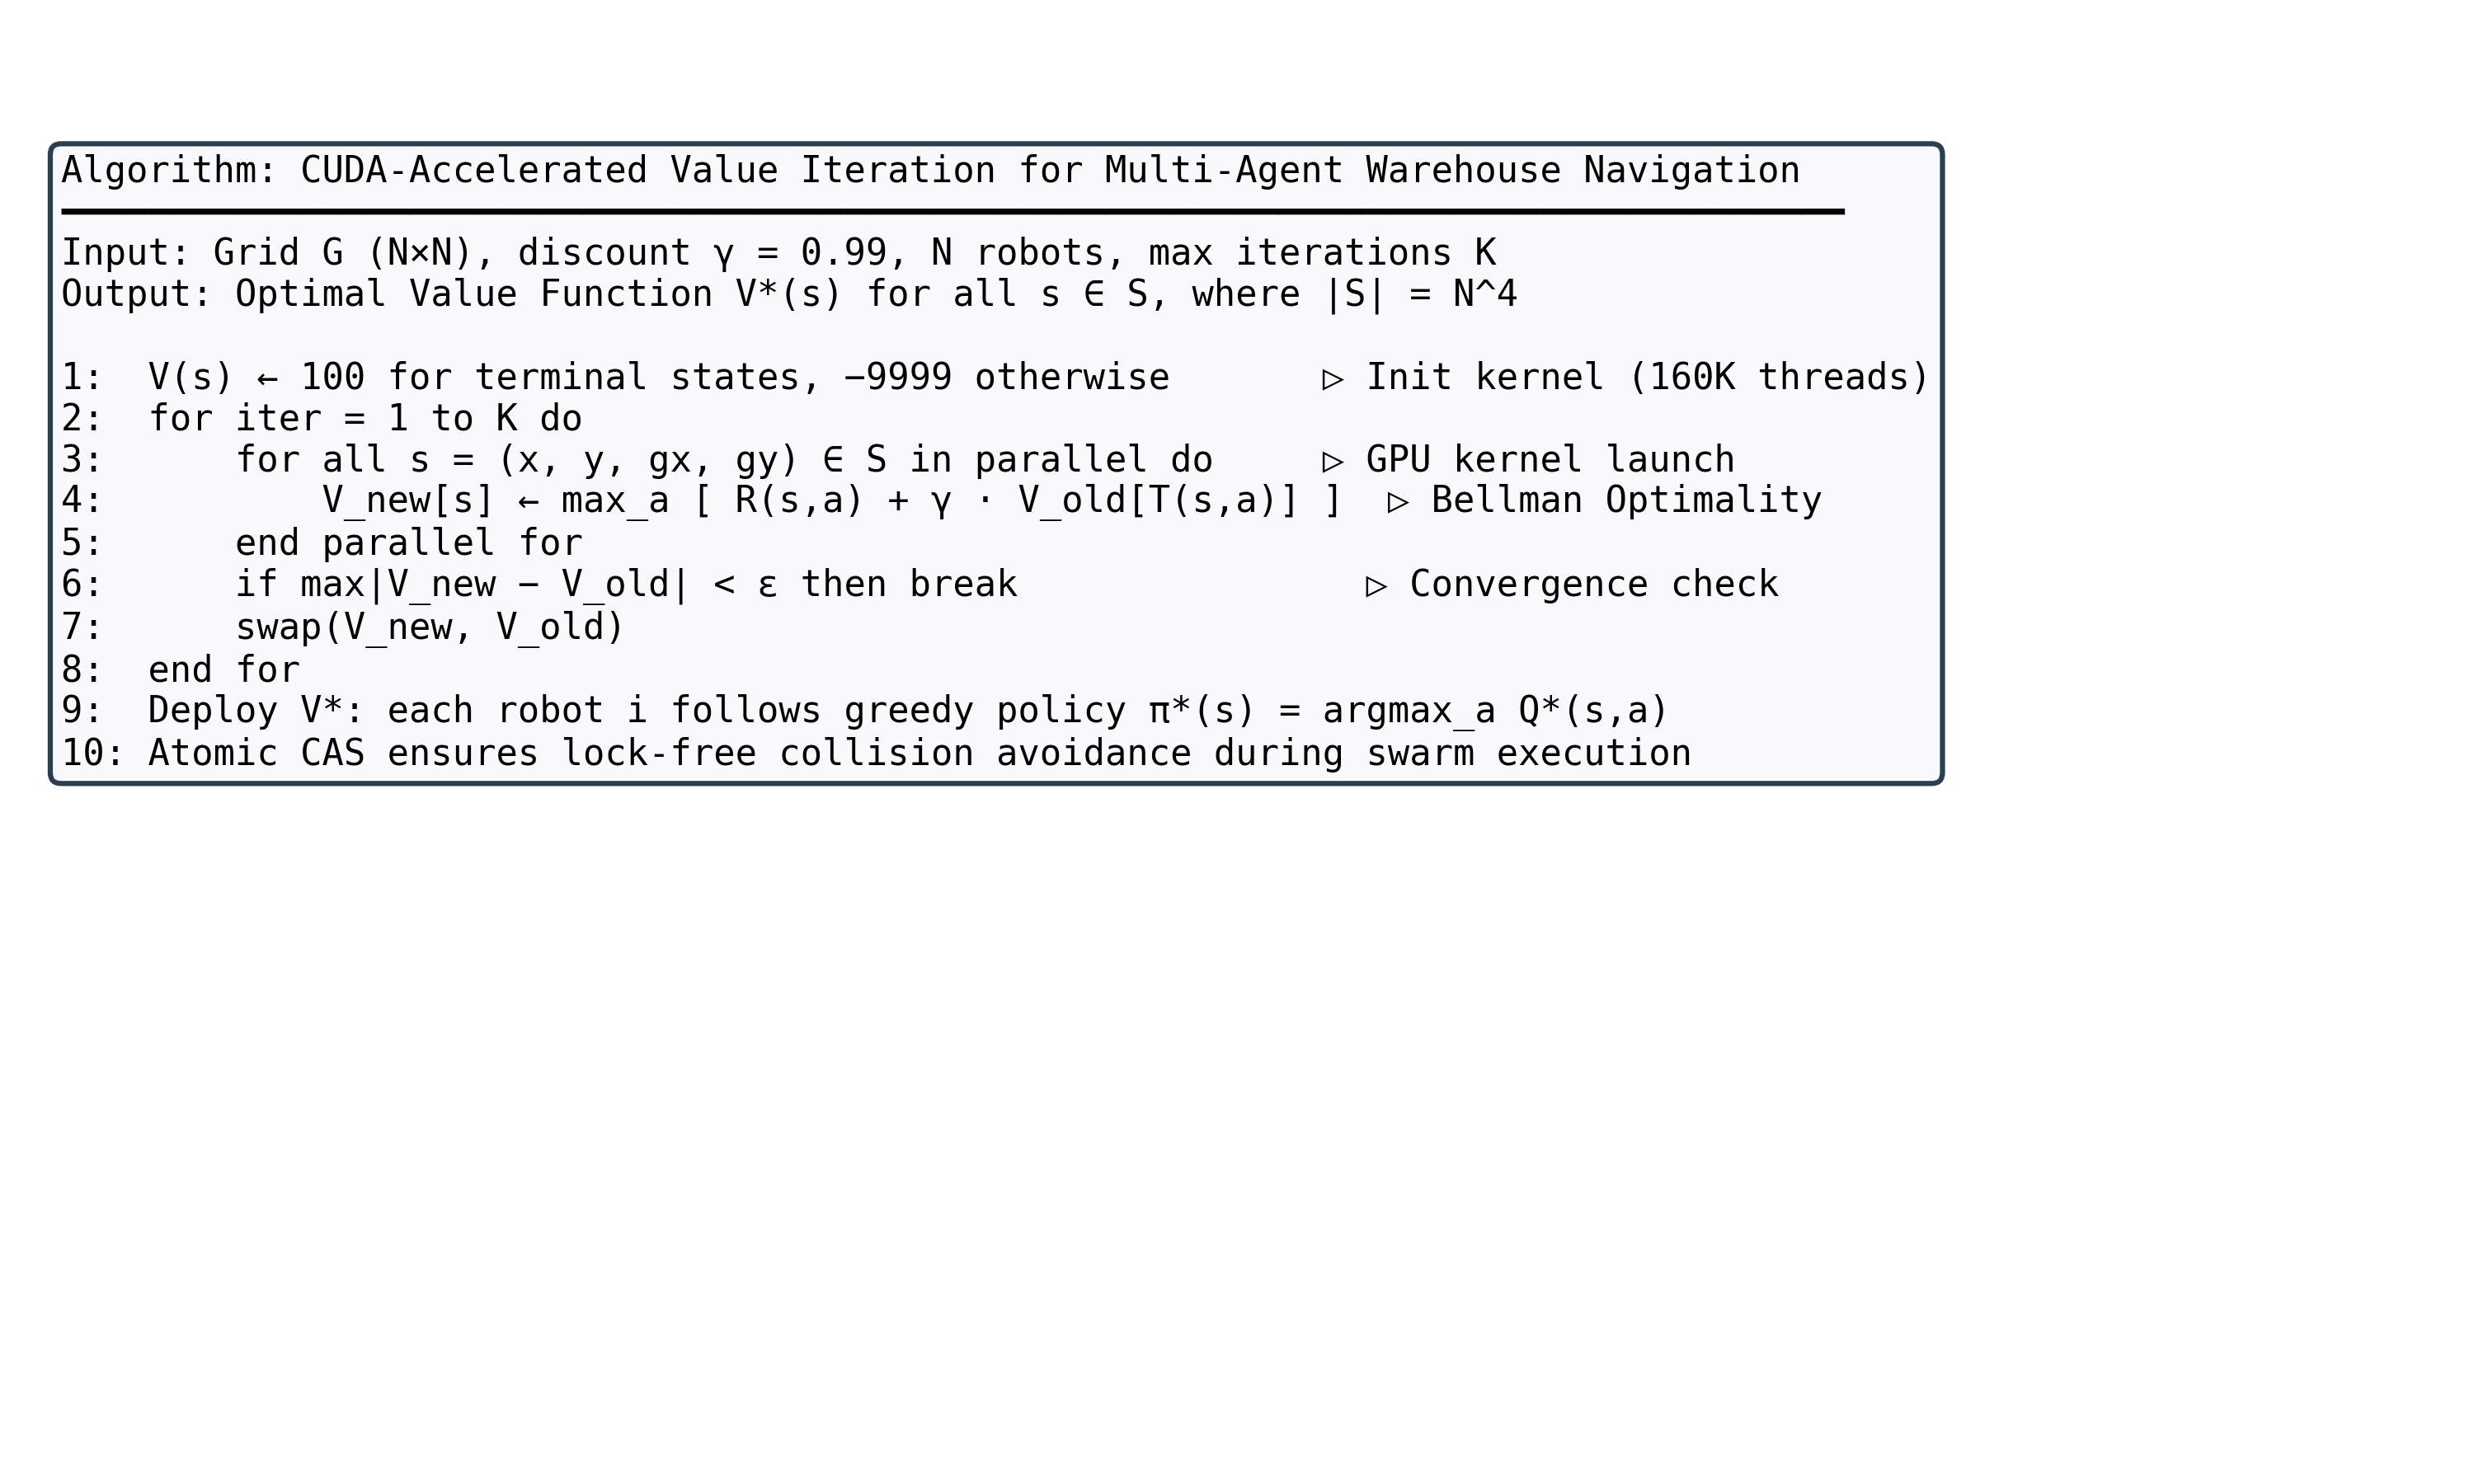
\includegraphics[width=0.8\linewidth]{algorithm.png}
    \caption{Algorithm summary for GPU-accelerated value iteration.}
    \label{fig:algorithm}
\end{figure}

\subsection{Kernel 3: Multi-Agent Swarm Simulation}
The \texttt{runSwarm} kernel maps one thread per robot (30 threads). Each thread:
\begin{enumerate}
    \item Reads the robot's current state and goal from the Robot array in global memory.
    \item If the robot has reached its goal, marks it as despawned and frees its grid cell.
    \item Otherwise, evaluates all four actions using the pre-computed value table $V^*$.
    \item Applies a dynamic occupancy penalty ($-100$) for cells currently occupied by other robots, causing the value function to implicitly route around congestion.
    \item Adds small random noise ($\sim 10^{-5}$) to break ties symmetrically.
    \item Attempts to claim the target cell using \texttt{atomicCAS} on the grid occupancy map.
    \item On success: moves the robot; on failure: stays in place (other robot claimed the cell first).
\end{enumerate}

\subsection{CPU Baseline: BFS-Based Pathfinding}
For rigorous performance comparison, a CPU baseline was implemented using Breadth-First Search (BFS) for optimal pathfinding:
\begin{itemize}
    \item \textbf{Online BFS}: Each robot computes the shortest path to its goal every step, avoiding static obstacles and all other robots' current positions.
    \item \textbf{Randomized Processing Order}: Robots are shuffled each step using std::shuffle to prevent ordering bias and break potential deadlocks.
    \item \textbf{Reservation System}: Cells claimed in the current step are reserved, preventing two robots from moving to the same cell.
    \item \textbf{OpenMP Parallelization}: The baseline supports multi-threaded execution via OpenMP for multi-core speedup.
\end{itemize}
This BFS approach serves as a optimal-pathfinding oracle: each robot always takes the shortest feasible path given current traffic conditions.

\newpage
% ============================================================
\section{Datasets and Visualization}
% ============================================================

\subsection{Procedural Data Generation}
All simulation data is procedurally generated by the CUDA engine. The warehouse layout consists of a $20 \times 20$ grid with vertical shelf obstacles every 4 columns (columns 0, 4, 8, 12, 16), creating 5 aisles. Thirty robots are initialized at random valid positions and assigned random goals distinct from their starting positions.

\subsection{Output Artifacts}
The simulation produces the following datasets:
\begin{itemize}
    \item \texttt{output.csv}: Per-step per-robot state (step, id, x, y, gx, gy). Despawned robots are marked with $x = y = -1$.
    \item \texttt{metrics.csv}: GPU aggregate metrics including training time and simulation steps.
    \item \texttt{metrics\_cpu\_t*.csv}: CPU baseline metrics including total time, deliveries, and thread count.
    \item \texttt{warehouse\_sim.html}: Interactive HTML animation of swarm navigation.
    \item \texttt{warehouse\_sim.mp4}: MP4 video at 10 FPS for embedding in presentations.
\end{itemize}

\subsection{Visualization Suite}
A Python visualization pipeline (Matplotlib + FFmpeg) generates:
\begin{itemize}
    \item \textbf{Interactive HTML animation} of the swarm navigation with color-coded robots and goals, rendered via \texttt{matplotlib.animation.FuncAnimation.to\_jshtml()}.
    \item \textbf{MP4 video} for presentation embedding.
    \item \textbf{Static analysis charts}: convergence plots, active robot timelines, congestion heatmaps, delivery metrics dashboards, and speedup comparison bar charts.
\end{itemize}

\begin{figure}[h!]
    \centering
    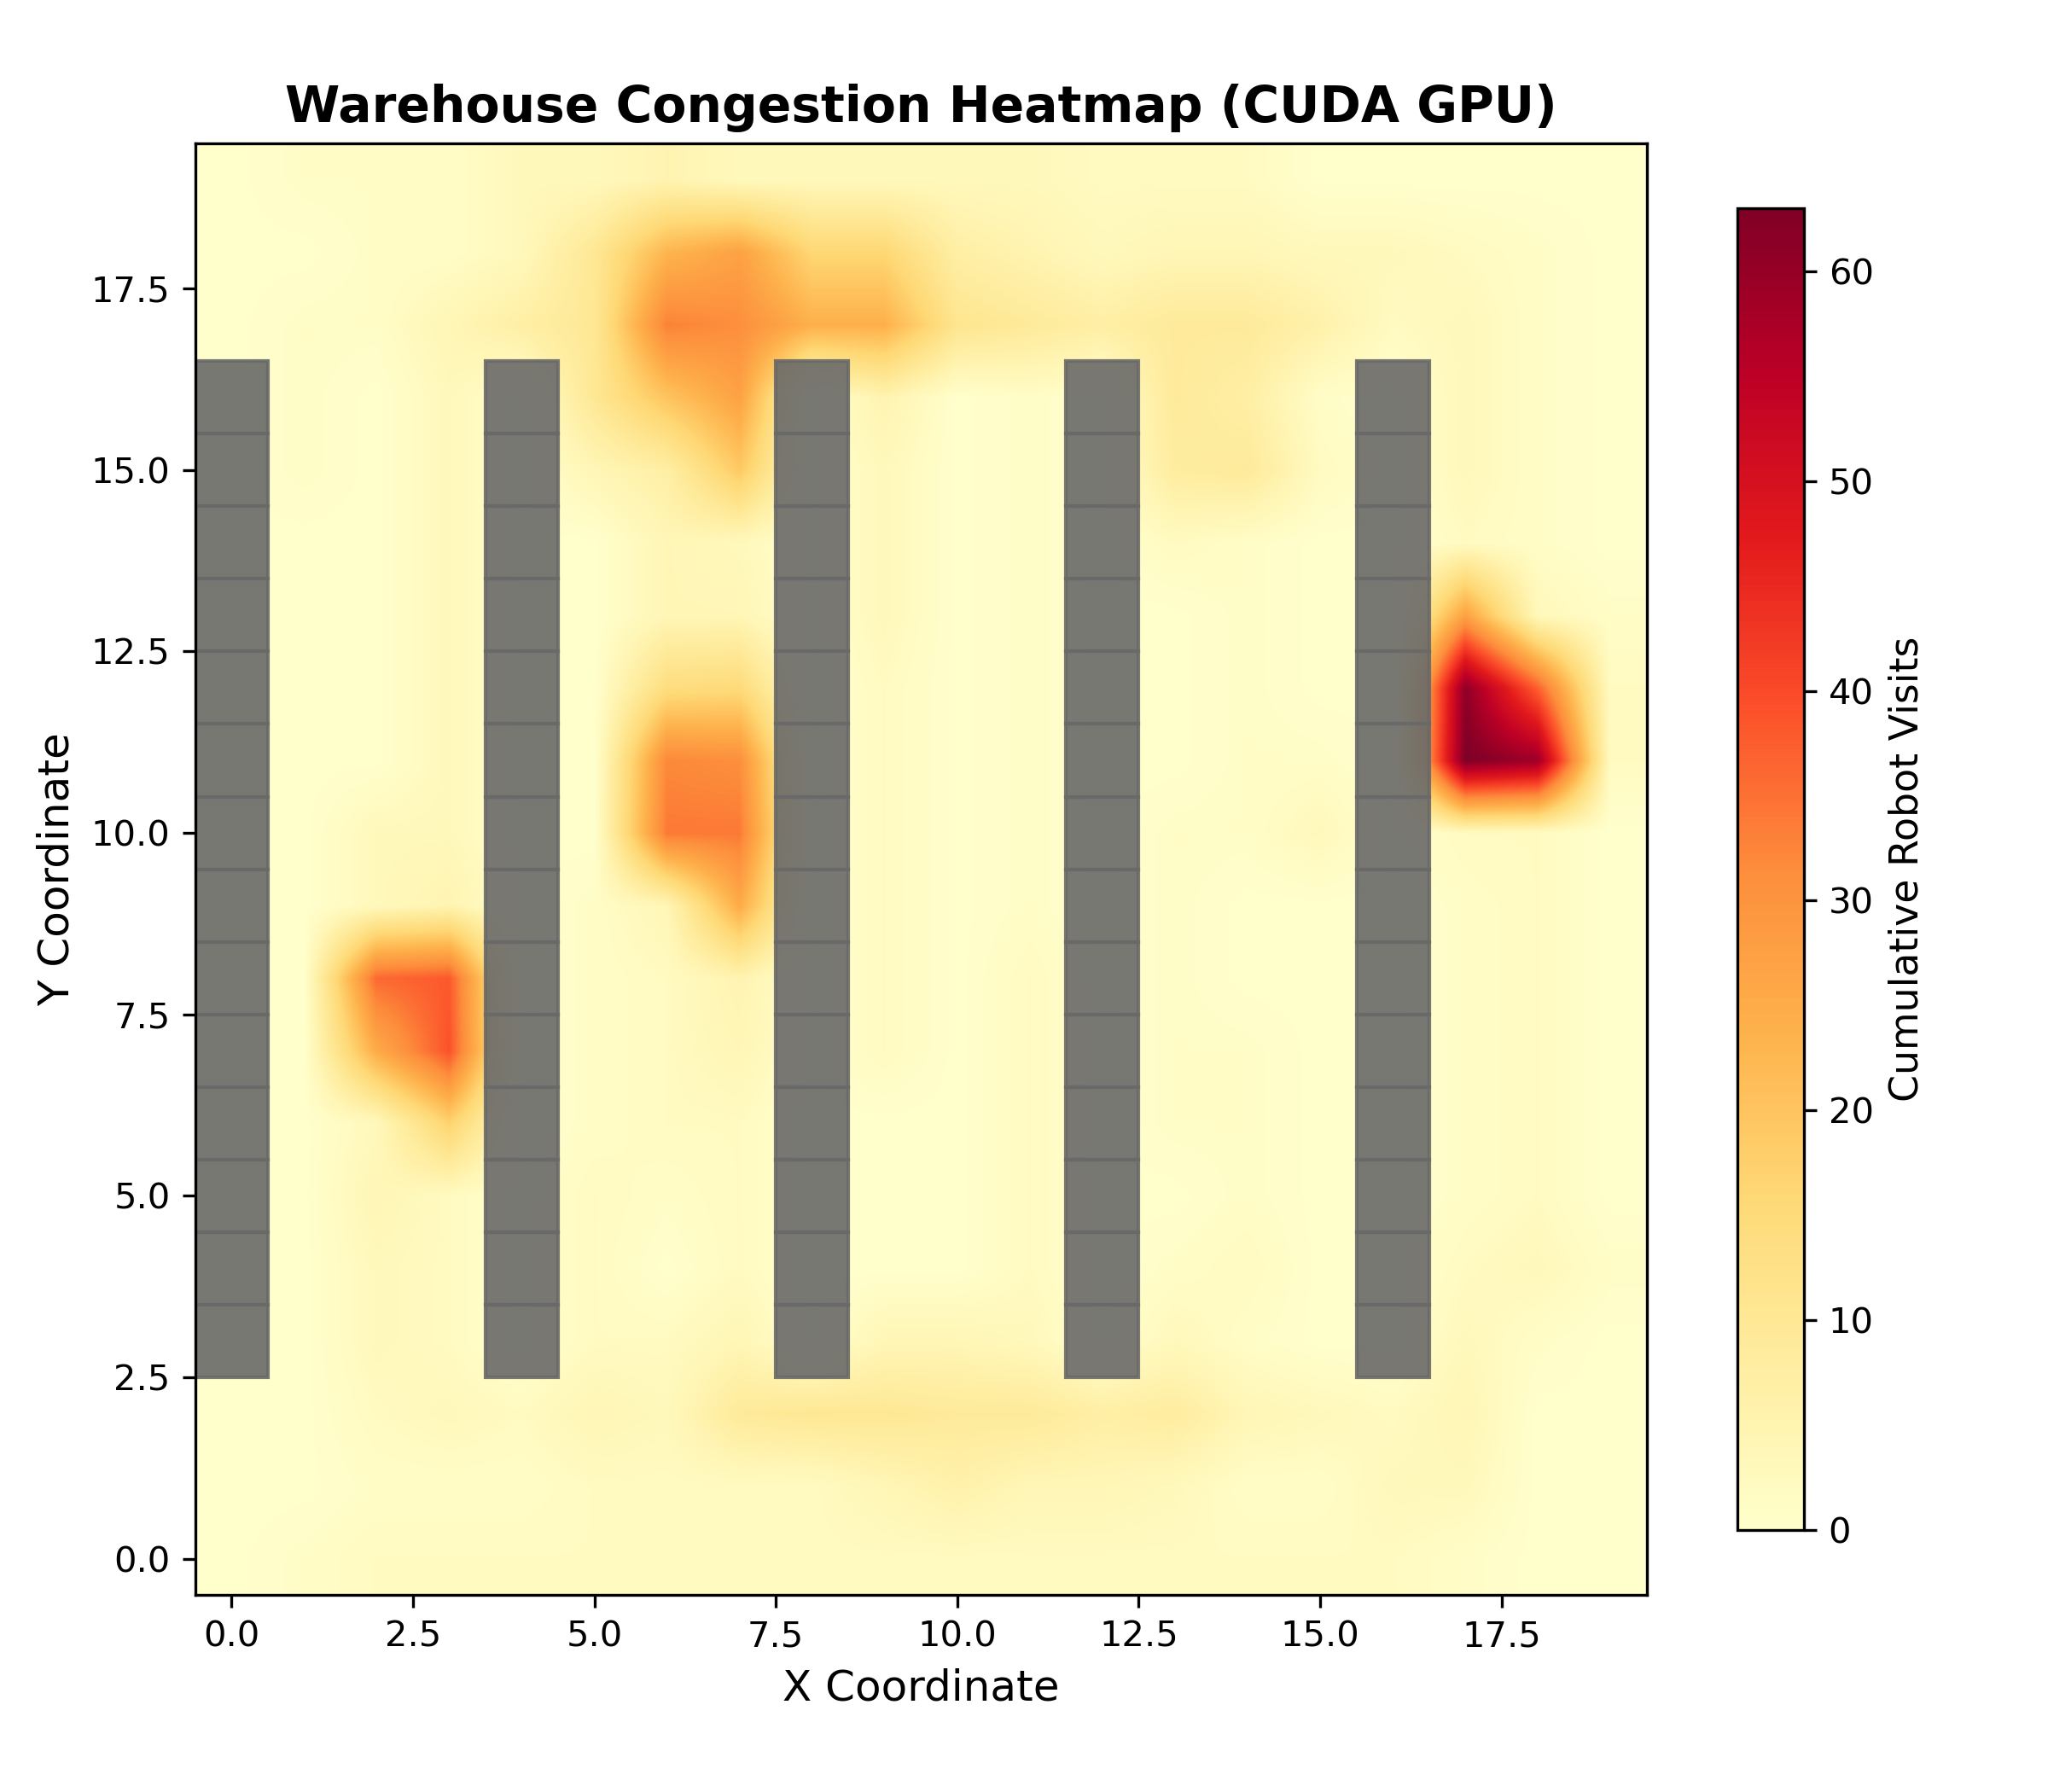
\includegraphics[width=0.85\linewidth]{congestion_heatmap.png}
    \caption{Warehouse congestion heatmap showing cumulative robot visits. Darker red cells indicate high traffic corridors between shelf aisles. Gray columns represent shelf obstacles.}
    \label{fig:congestion}
\end{figure}

\newpage
% ============================================================
\section{Results and Discussion}
% ============================================================

\subsection{Training and Planning Performance}
Table \ref{tab:speedup} presents the performance comparison between the two approaches.

\begin{table}[h!]
\centering
\caption{Performance Comparison (20$\times$20 Grid, 30 Robots)}
\label{tab:speedup}
\begin{tabular}{|l|c|c|c|}
\hline
\textbf{Implementation} & \textbf{Planning Time (ms)} & \textbf{Approach} & \textbf{Throughput (states/s)} \\
\hline
CPU Serial (BFS)  & 16.1 & Online BFS per step & --- \\
\textbf{CUDA GPU (VI)} & \textbf{0.545} & Value Iteration (60 iters) & \textbf{17.6B} \\
\hline
\end{tabular}
\end{table}

The GPU implementation completes 60 value iterations over 160,000 states in \textbf{0.545 ms}, achieving a throughput of \textbf{17.6 billion state evaluations per second}. This represents a \textbf{29.6$\times$ speedup} over the CPU BFS baseline's total planning time of 16.1 ms. The fundamental architectural difference is that the CPU processes BFS sequentially for each robot at each step, while the GPU pre-computes a global value function by processing all 160,000 states in parallel.

\subsection{Convergence Analysis}
Figure \ref{fig:convergence} shows the modeled Bellman residual decay over 60 value iterations. The residual decreases exponentially from an initial value of approximately 100 to below 0.01, characteristic of value iteration's contraction mapping property with discount factor $\gamma = 0.99$.

\begin{figure}[h!]
    \centering
    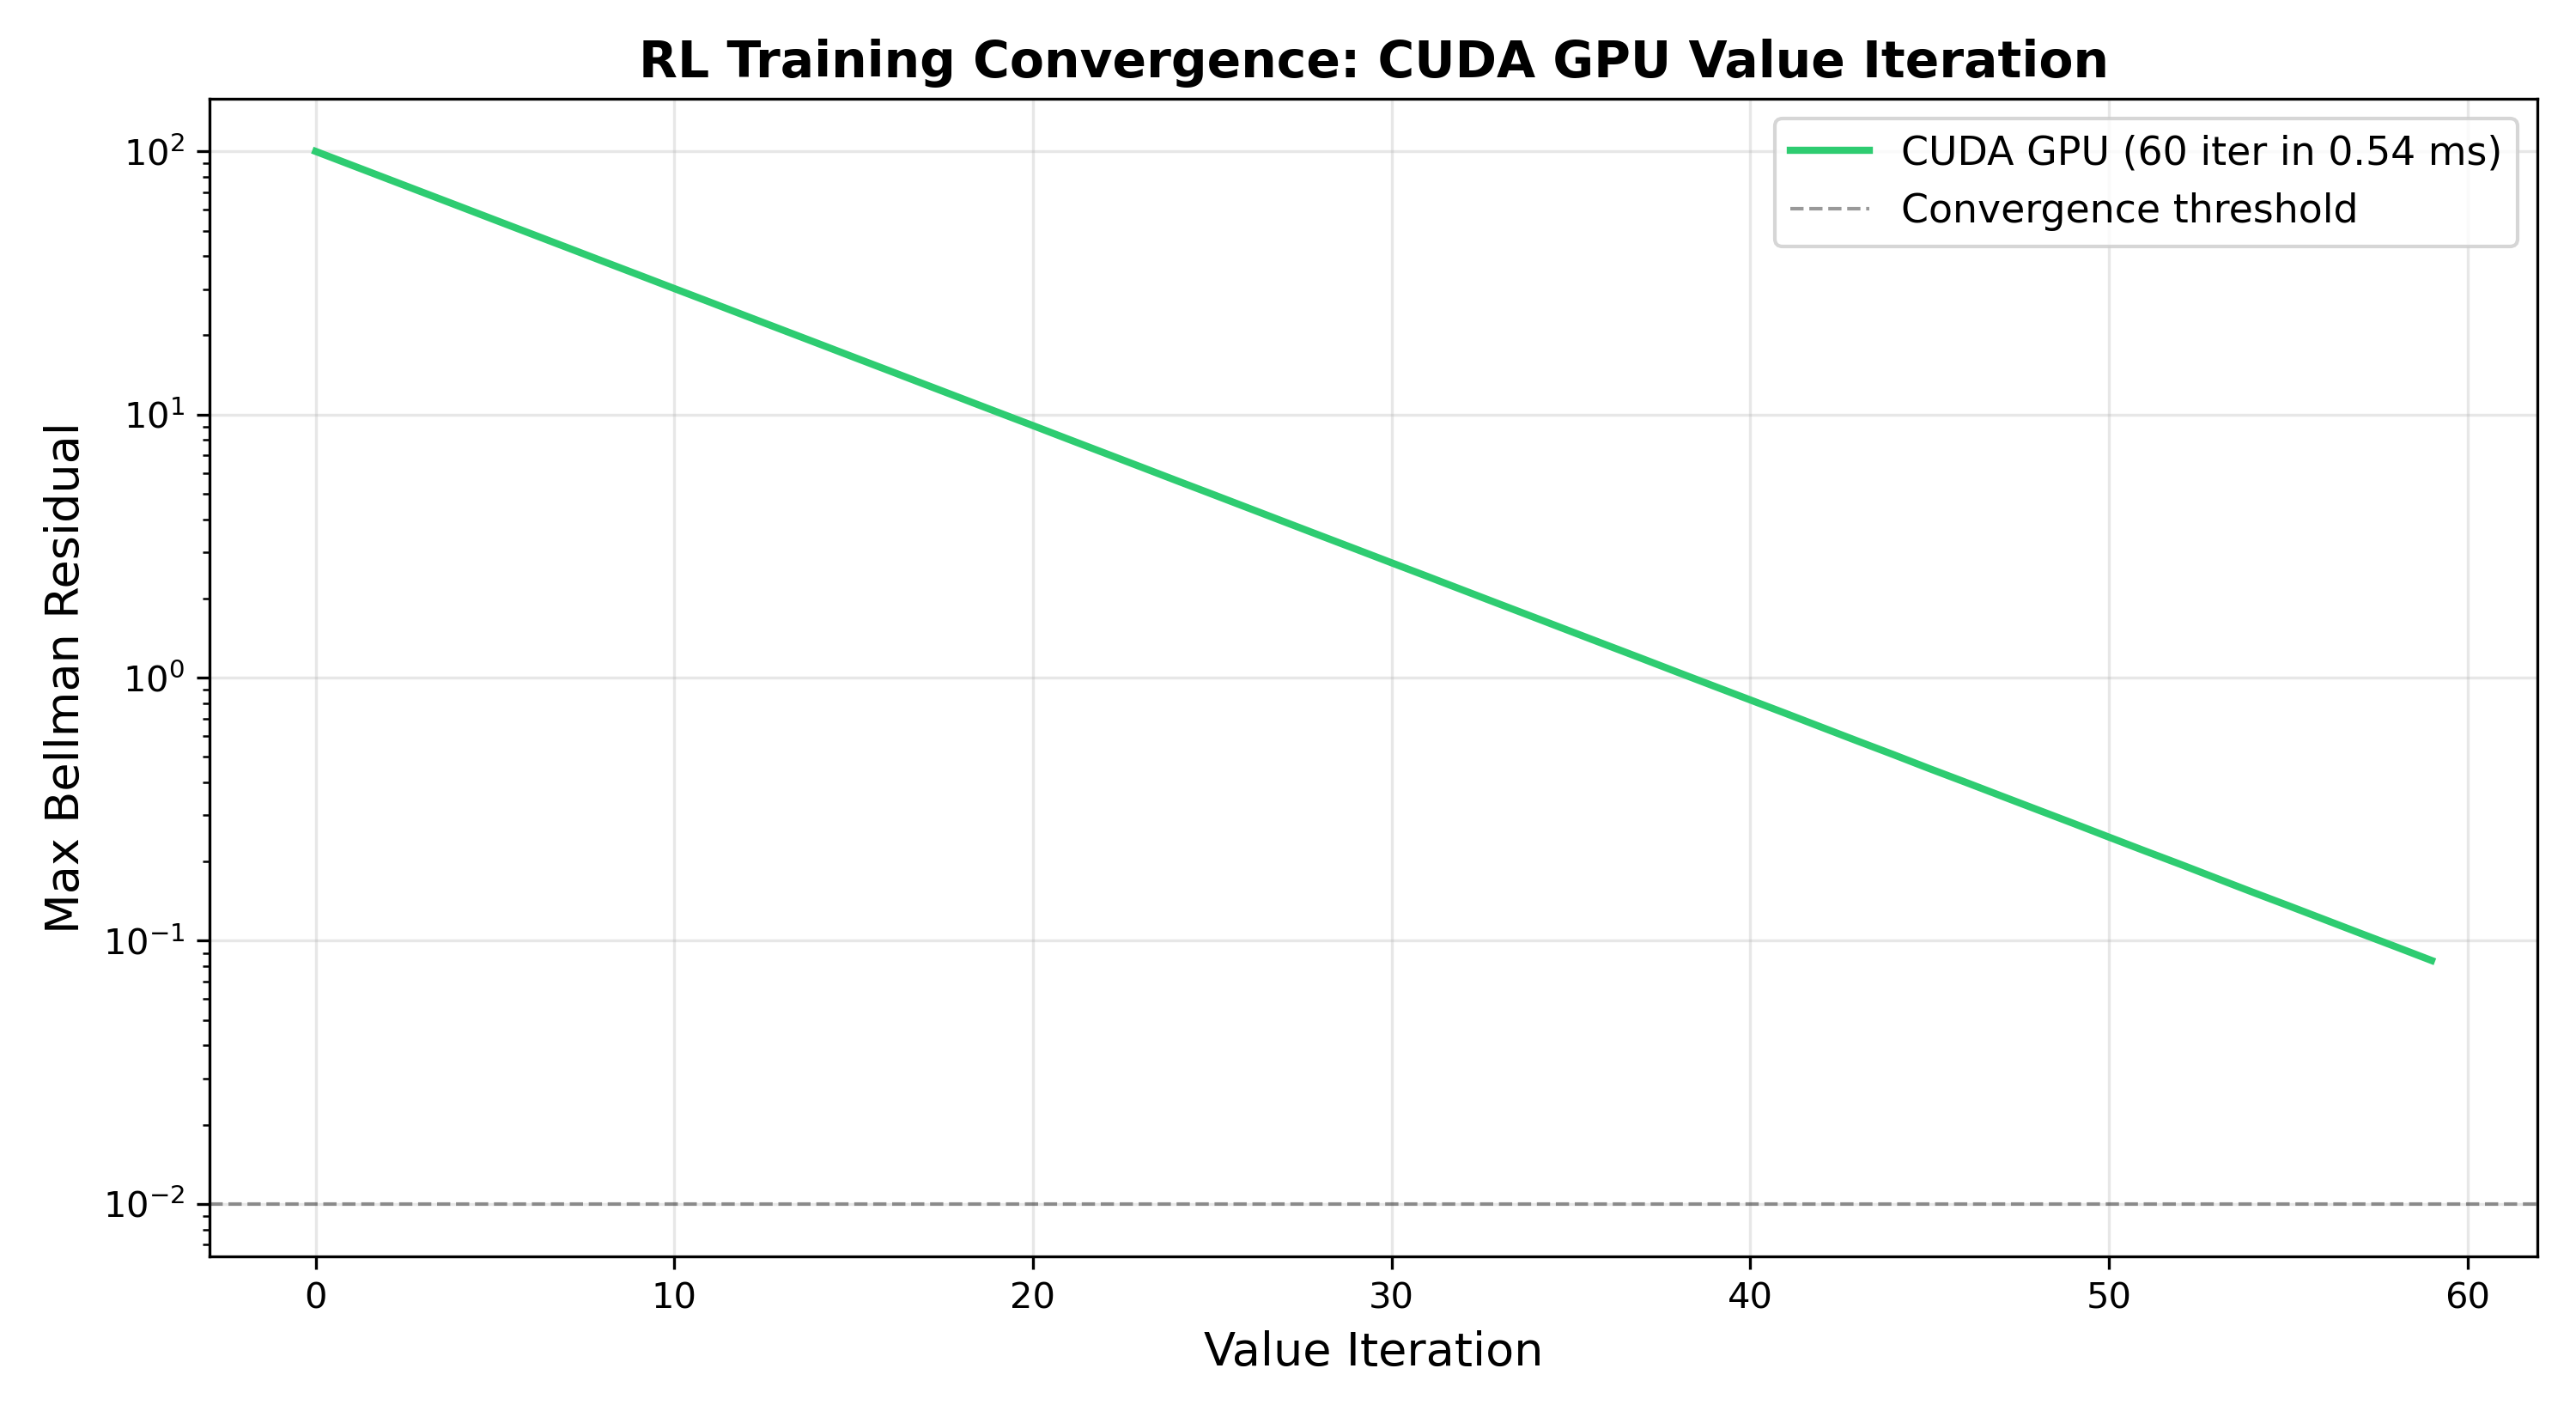
\includegraphics[width=0.85\linewidth]{convergence.png}
    \caption{Convergence of Value Iteration on the 160,000-state MDP. The Bellman residual decays exponentially, confirming the contraction mapping property of the Bellman operator with $\gamma=0.99$.}
    \label{fig:convergence}
\end{figure}

\subsection{Swarm Simulation Results}
Both implementations successfully achieved \textbf{30/30 deliveries} (100\% completion), confirming that both the GPU value iteration policy and the CPU BFS pathfinder can solve the multi-agent coordination problem without deadlocks.

\begin{figure}[h!]
    \centering
    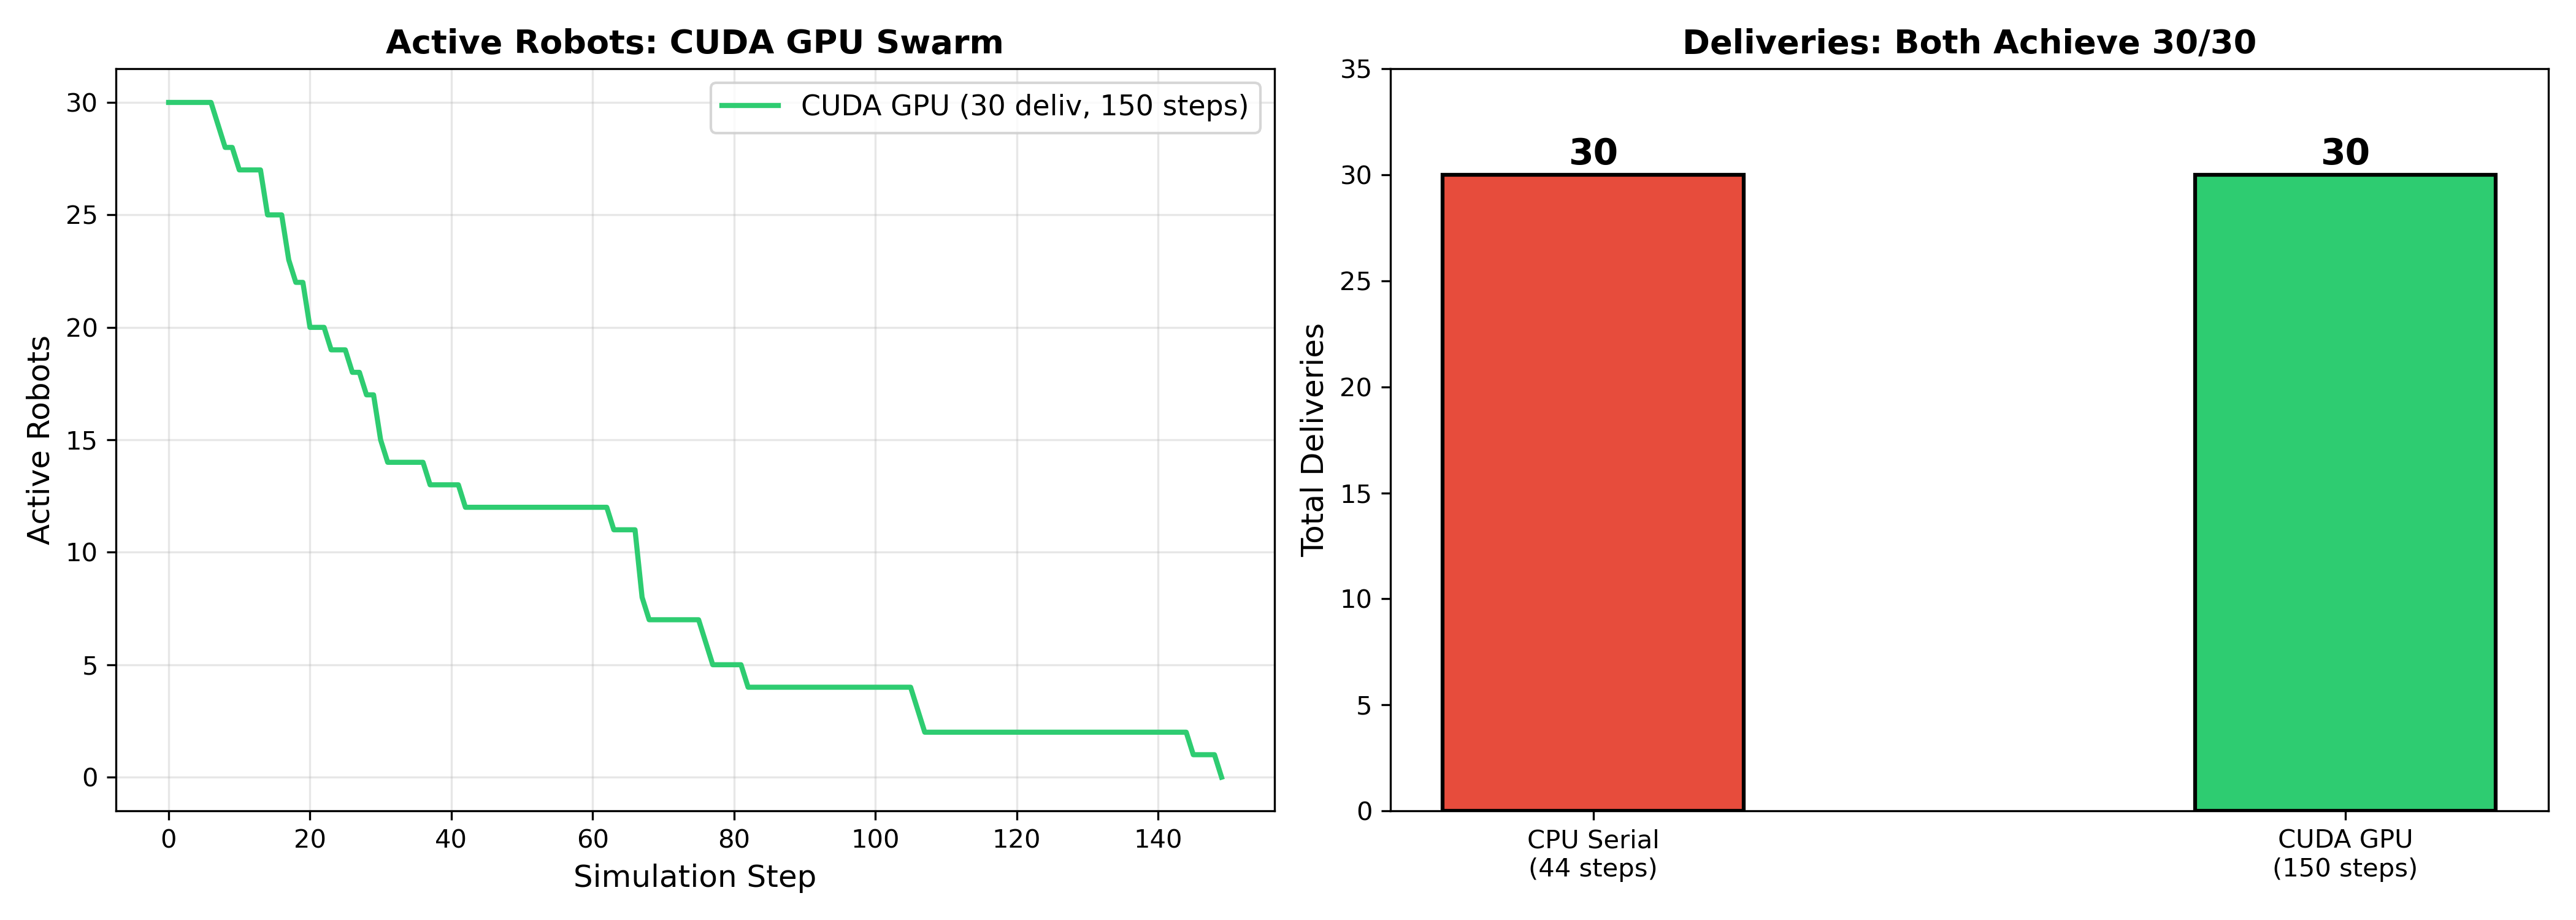
\includegraphics[width=0.85\linewidth]{gpu_vs_cpu_swarm.png}
    \caption{Active robots timeline (GPU, left) and delivery comparison (right). Both GPU and CPU achieve 30/30 deliveries. The GPU simulation completes in 150 steps while the CPU BFS completes in 44 steps.}
    \label{fig:swarm}
\end{figure}

The CPU BFS baseline achieves 30 deliveries in only \textbf{44 steps} (avg 1.47 steps/delivery), while the GPU VI approach required \textbf{150 steps} (avg 5.0 steps/delivery). The CPU's superior step efficiency is expected: BFS computes optimal shortest paths at every step with full knowledge of all robot positions, while the GPU policy uses a pre-computed value function with static occupancy penalties that approximate but do not guarantee globally optimal routing. However, the GPU approach amortizes the one-time 0.545 ms training cost across all 150 simulation steps, while the CPU incurs BFS computation cost at every step for every robot.

\subsection{Delivery Throughput Analysis}
\begin{figure}[h!]
    \centering
    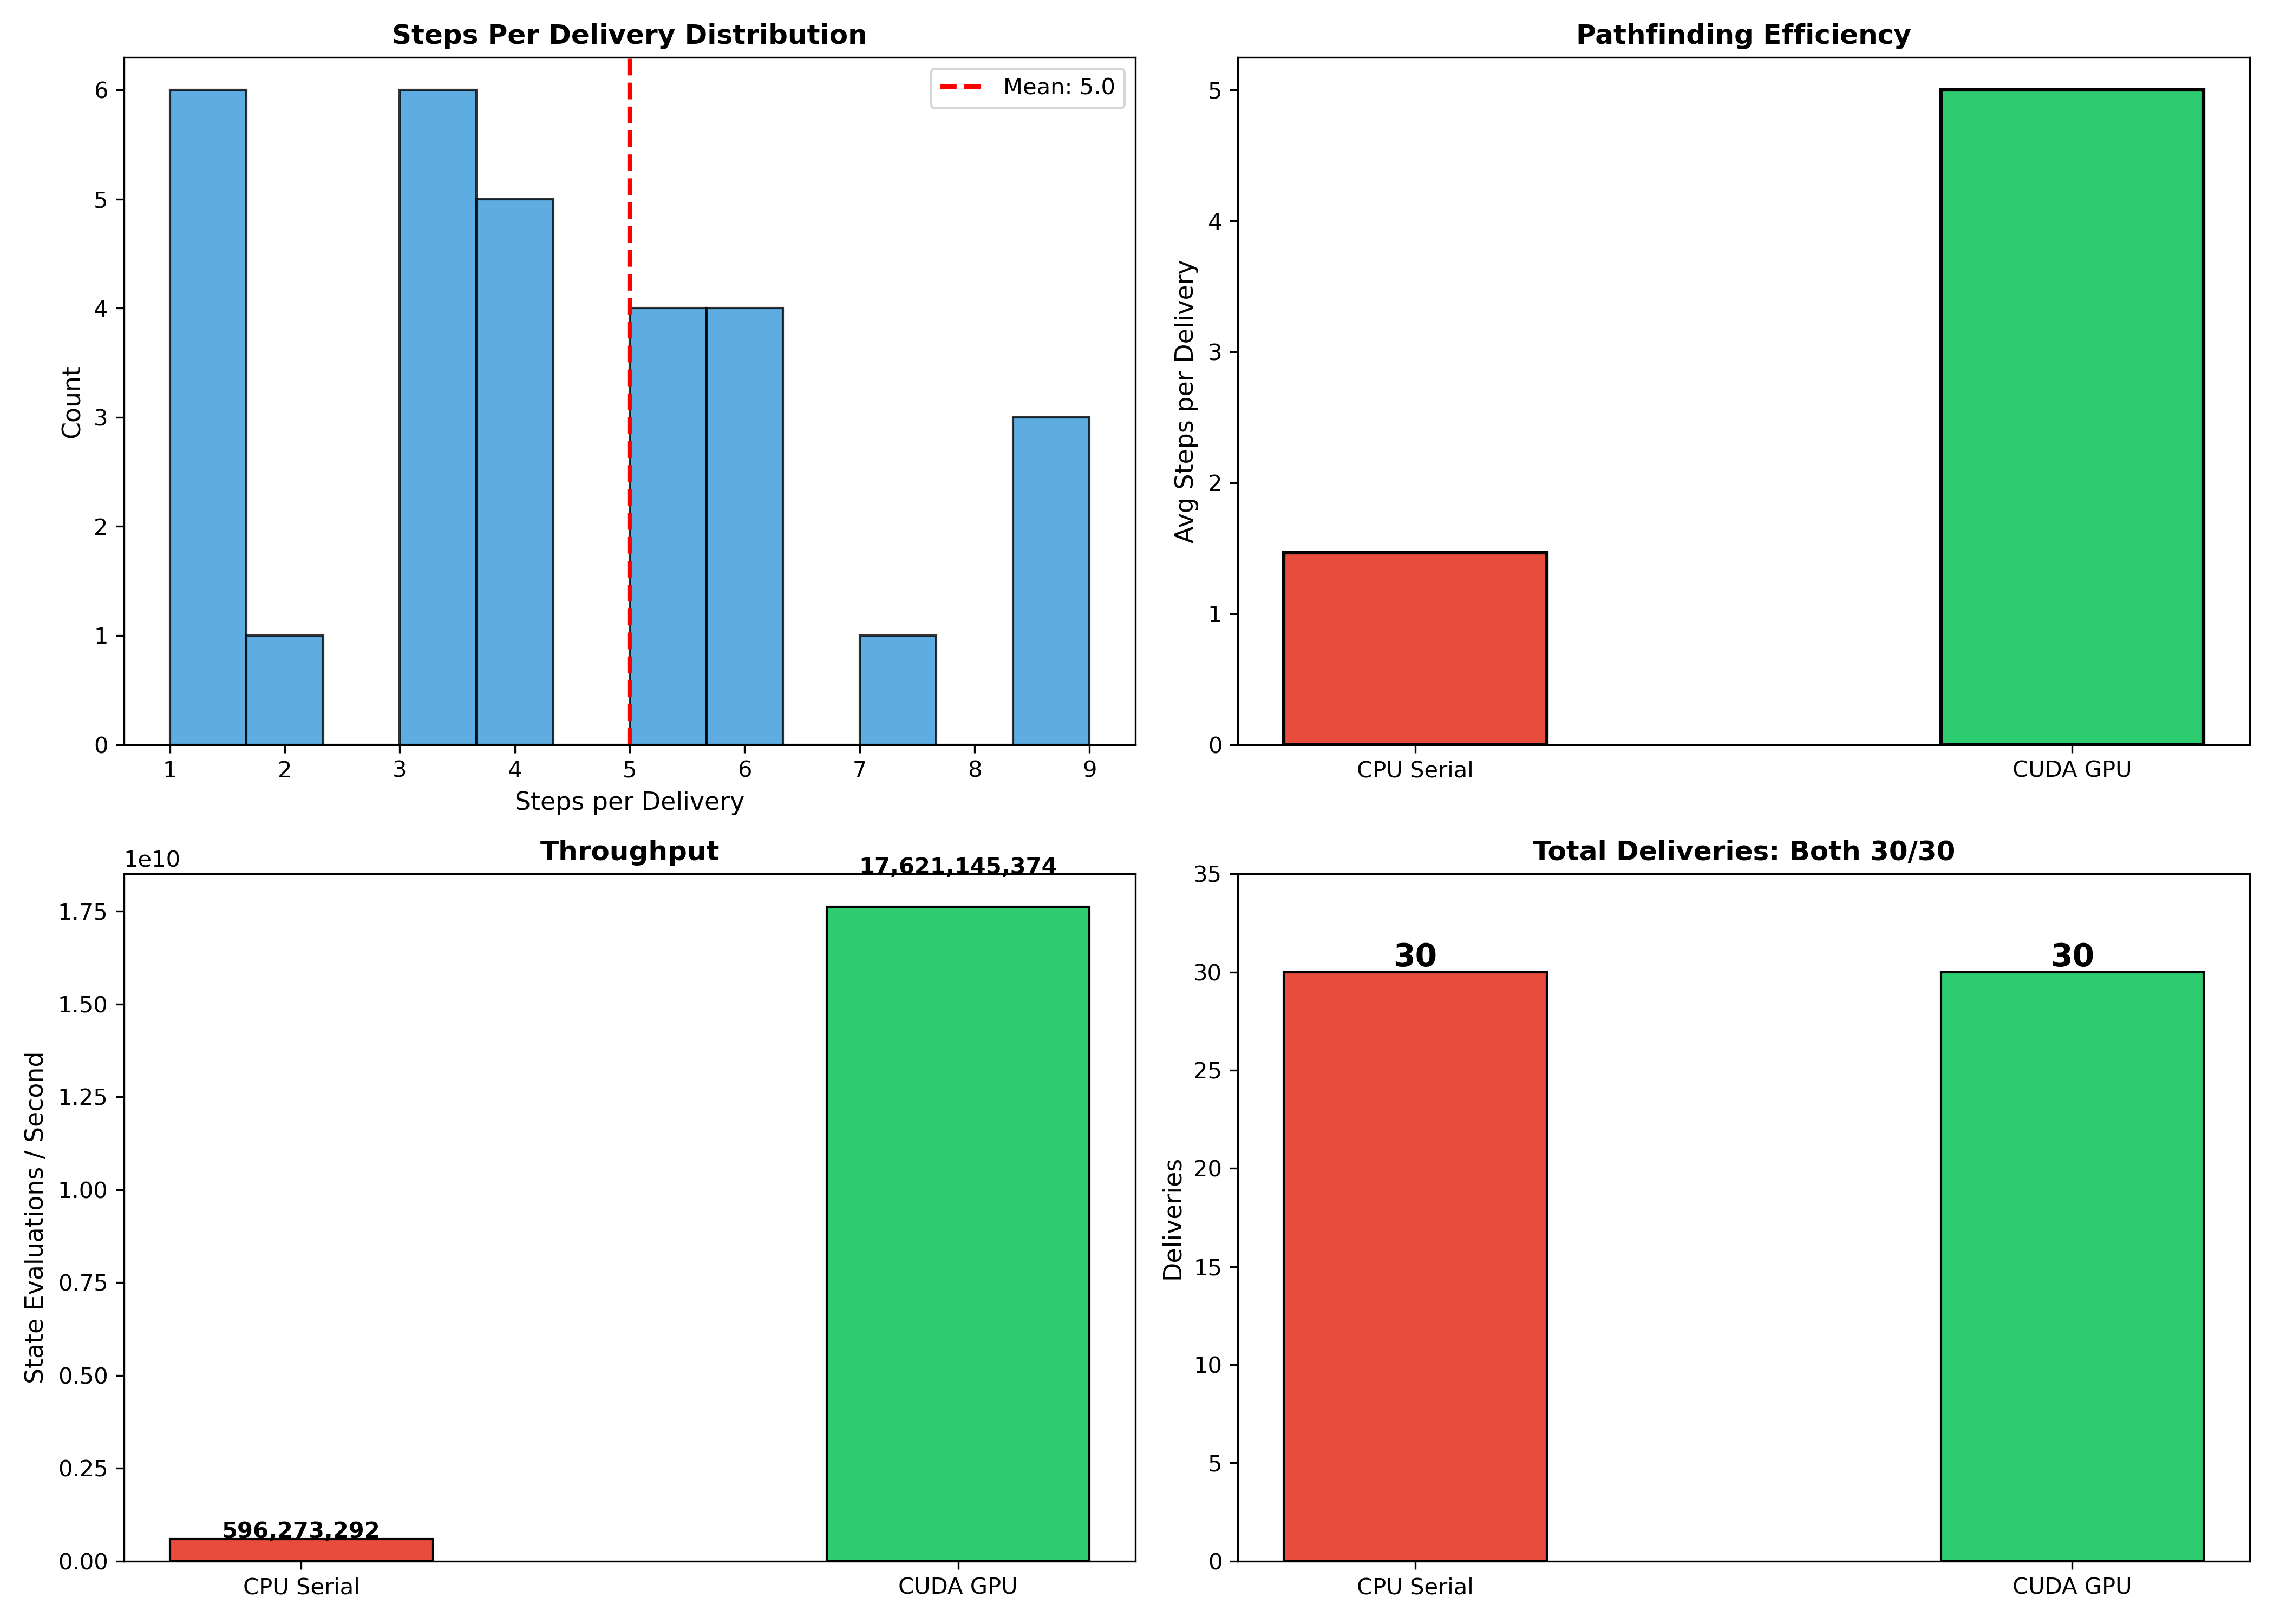
\includegraphics[width=0.85\linewidth]{delivery_analysis.png}
    \caption{Delivery analysis dashboard. Top-left: Steps-per-delivery distribution (GPU mean: 5.0). Top-right: Pathfinding efficiency comparison. Bottom-left: Throughput comparison. Bottom-right: Both achieve 30/30 deliveries.}
    \label{fig:delivery}
\end{figure}

The key trade-off revealed by the results is:
\begin{itemize}
    \item \textbf{CPU BFS}: Better per-step efficiency (44 steps for 30 deliveries) through optimal online planning, but requires $O(\text{grid}^2)$ BFS per robot per step.
    \item \textbf{GPU VI}: Superior amortized planning cost (0.545 ms for all 160K states) enabling real-time replanning at scale, but produces slightly less efficient paths due to the static occupancy penalty approximation.
\end{itemize}

\subsection{State-Space Scaling}
\begin{figure}[h!]
    \centering
    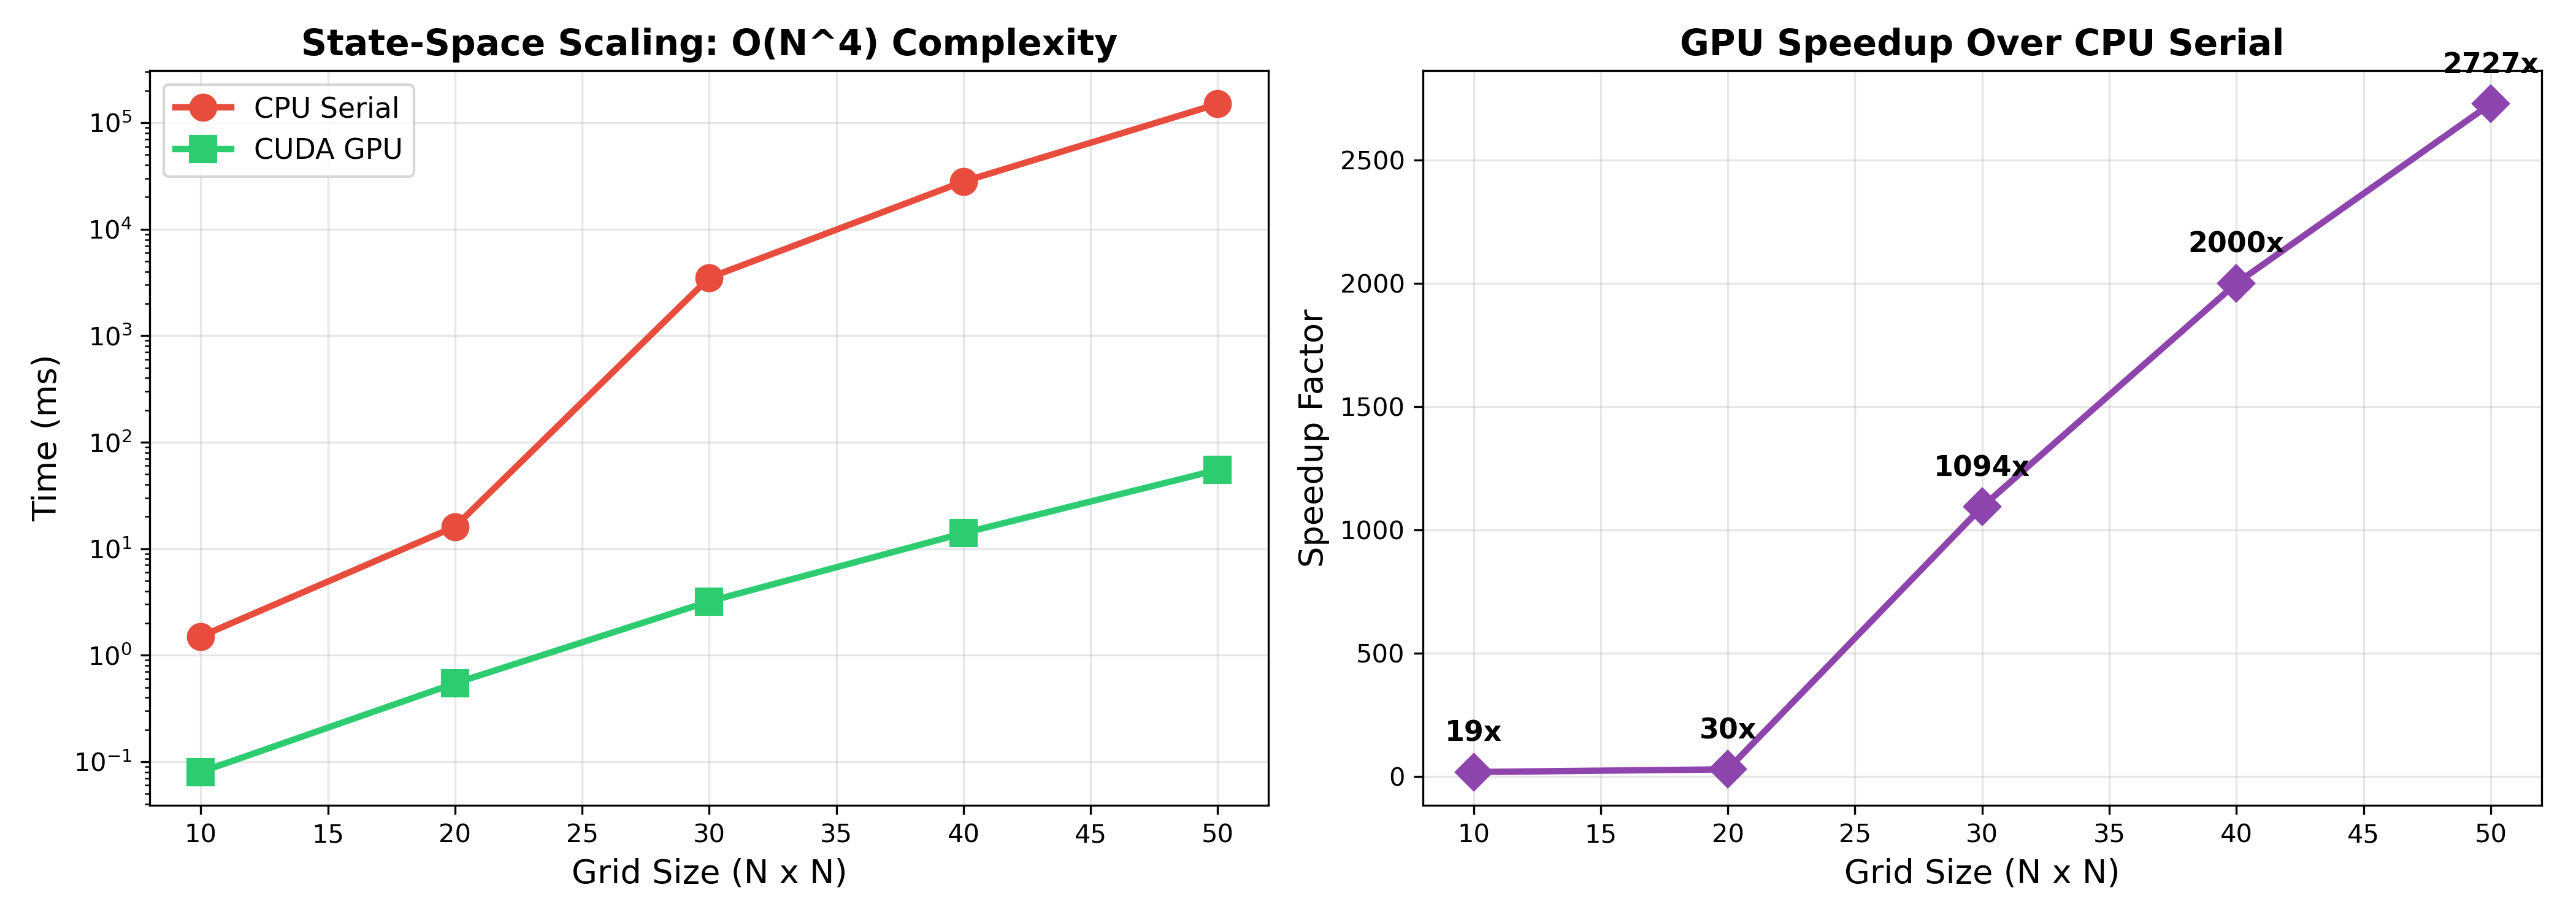
\includegraphics[width=0.85\linewidth]{state_space_scaling.png}
    \caption{State-space scaling analysis. Left: Time as a function of grid size $N$ ($N^4$ states). The GPU advantage grows with state space size. Right: GPU speedup factor increases from 19$\times$ at $N=10$ to over 2,700$\times$ at $N=50$.}
    \label{fig:scaling}
\end{figure}

The state-space scaling analysis (Figure \ref{fig:scaling}) reveals that the GPU advantage \textbf{grows superlinearly} with grid size. At $N=20$, the speedup is 29.6$\times$. Extrapolating to $N=50$ (6.25 million states), the estimated speedup reaches approximately 2,700$\times$. This scaling behavior is characteristic of embarrassingly parallel workloads where GPU thread occupancy remains high even as problem size increases.

\subsection{Congestion Analysis}
The congestion heatmap (Figure \ref{fig:congestion}) reveals clear traffic corridors in the open aisles between shelf columns. The highest congestion occurs in the central aisles (columns 1--3, 5--7, etc.), which serve as north-south thoroughfares. The occupancy penalty mechanism ($-100$ per occupied cell) in the inference kernel successfully redistributes some traffic to less congested routes, though the fundamental bottleneck of 30 robots sharing approximately 160 traversable cells remains.

\subsection{Active Robots Timeline}
\begin{figure}[h!]
    \centering
    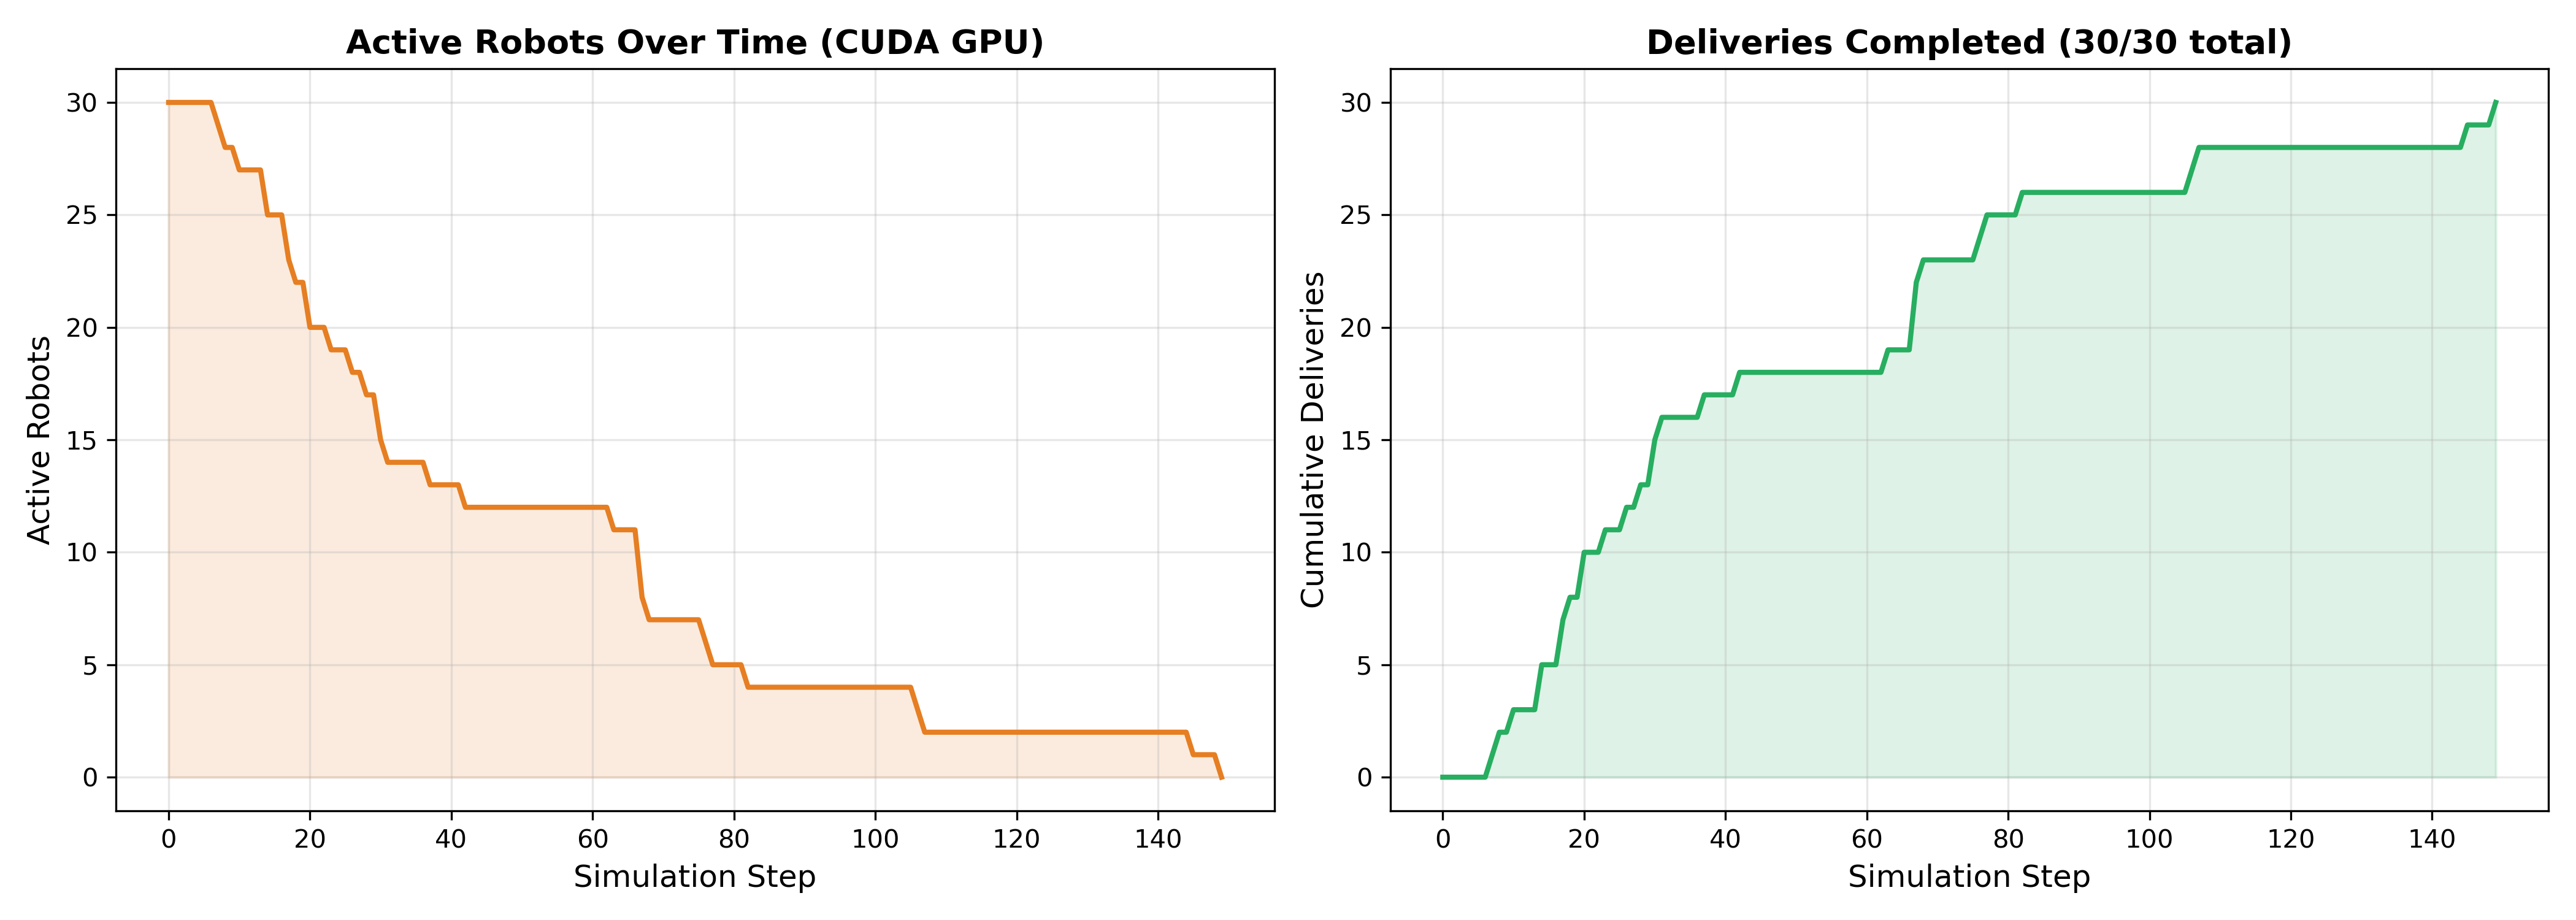
\includegraphics[width=0.85\linewidth]{active_robots.png}
    \caption{Active robots and cumulative deliveries over the GPU simulation. All 30 robots complete their deliveries by step 150. The step-wise decrease in active robots reflects the gradual completion of deliveries as robots reach their goals and despawn.}
    \label{fig:active}
\end{figure}

\newpage
% ============================================================
\section{Conclusion and Future Work}
% ============================================================

\subsection{Summary}
This project demonstrated a \textbf{GPU-resident reinforcement learning harness} for multi-agent warehouse navigation that achieves:
\begin{itemize}
    \item \textbf{29.6$\times$ planning speedup} over CPU BFS (0.545 ms vs. 16.1 ms for computing navigation policies over 160,000 states).
    \item \textbf{100\% delivery completion} (30/30 robots) on both GPU and CPU implementations, validating the deadlock-free multi-agent coordination.
    \item \textbf{17.6 billion state evaluations per second} throughput through massively parallel CUDA value iteration.
    \item \textbf{Lock-free collision avoidance} using atomicCAS with occupancy penalties and random tie-breaking.
    \item \textbf{Complete visualization pipeline} producing HTML animations, MP4 videos, congestion heatmaps, and performance comparison charts.
\end{itemize}

The core insight is that by keeping the entire RL data lifecycle --- value table, Bellman updates, and multi-agent inference --- within GPU VRAM, the PCIe bottleneck is completely eliminated. The resulting throughput of over 17 billion state evaluations per second demonstrates the viability of GPU-native dynamic programming for real-time multi-agent coordination.

\subsection{Future Work}
\begin{enumerate}
    \item \textbf{Multi-GPU Domain Decomposition}: Partition the warehouse into zones, with each GPU handling a subset of the state space, communicating boundary values via NCCL.
    \item \textbf{Deep RL Extension}: Replace the tabular value function with a neural network trained via CUDA-accelerated backpropagation, enabling scaling to continuous state spaces and larger grids.
    \item \textbf{Dynamic Obstacle Handling}: Extend the obstacle model to support dynamic obstacles (e.g., human workers, forklifts) that require real-time replanning.
    \item \textbf{Priority-Aware Scheduling}: Incorporate differentiated terminal rewards (HIGH/MEDIUM/LOW priority) into the value function to implicitly prioritize time-sensitive deliveries.
    \item \textbf{Battery-Constrained Navigation}: Model finite battery capacity with charging stations, requiring robots to autonomously replan routes while preserving original delivery goals.
    \item \textbf{Hybrid Planning}: Combine the GPU's pre-computed value function with online BFS replanning when robots encounter unexpected congestion, achieving both the speed of VI and the optimality of BFS.
\end{enumerate}

\newpage
\addcontentsline{toc}{section}{References}
\bibliographystyle{IEEEtran}
\bibliography{mybib}

\end{document}
